\emph{Cet exercice est un questionnaire à choix multiples. Pour chaque question, une seule des quatre propositions est exacte. Indiquer sur la copie le numéro de la question et la lettre de la proposition choisie. Aucune justification n'est demandée.\\
Pour chaque question, une réponse exacte rapporte un point. Une réponse fausse, une réponse multiple ou l'absence de réponse ne rapporte ni n'enlève de point.}

\bigskip

\textbf{Question 1 :}

\smallskip

On considère la suite numérique $\left(u_n\right)$ définie pour tout $n$ entier naturel par $u_n = \frac{1+2^n}{3+5^n}$. Cette suite :

\medskip

\begin{tblr}{width=\linewidth,colspec={X[l,m]X[l,m]}}%X[l,m]X[l,m]}}
	(a)~~diverge vers $+\infty$ & (b)~~converge vers $\tfrac{2}{5}$ \\
	(c)~~converge vers 0 & (d)~~converge vers $\tfrac{1}{3}$
\end{tblr}

\bigskip

\textbf{Question 2 :}

\medskip

Soit $f$ la fonction définie sur $]0;+\infty[$ par $f(x) x^2\,\ln(x)$. L'expression de la fonction dérivée de $f$ est :

\medskip

\begin{tblr}{width=\linewidth,colspec={X[l,m]X[l,m]}}%X[l,m]X[l,m]}}
	(a)~~$f'(x)=2x\,\ln(x)$ & (b)~~$f'(x)=x(2\,\ln(x)+1)$ \\
	(c)~~$f'(x)=2$ & (d)~~$f'(x)=x$
\end{tblr}

\bigskip

\textbf{Question 3 :}

\medskip

On considère une fonction $h$ dont le tableau de variation est donné ci-dessous : 

\begin{center}
	\begin{tikzpicture}
		\tkzTabInit[espcl=6]{$x$/1,$h$/2}{$-\infty$,$+\infty$}
		\tkzTabVar{-/$-\infty$,+/$+\infty$}
		\tkzTabVal{1}{2}{0.5}{$1$}{$0$}
	\end{tikzpicture}
\end{center}

On note $H$ la primitive de $h$ définie sur $\mathbb{R}$ qui s'annule en 0. Elle vérifie la propriété :

\medskip

\begin{tblr}{width=\linewidth,colspec={X[l,m]X[l,m]}}
	(a)~~$H$ positive sur $]-\infty;0]$ & (b)~~$H$ négative sur $]-\infty;1]$ \\ (c)~~$H$ croissante sur $]-\infty;1]$ & (d)~~$H$ croissante sur $\mathbb{R}$
\end{tblr}

\bigskip

\textbf{Question 4 :}

\medskip

Soit deux réels $a$ et $b$ avec $a < b$.

On considère une fonction $f$ définie, continue, strictement croissante sur l'intervalle $[a;b]$ et qui s'annule en un réel $\alpha$.

Parmi les propositions suivantes, la fonction en langage \textsf{Python} qui permet de donner une valeur approchée de $\alpha$ à $0,001$ est :

\medskip

\begin{tblr}{width=\linewidth,colspec={X[l,m]X[l,m]}}
	(a)~~ & (b)~~
\end{tblr}

\begin{minipage}{0.5\linewidth}
\begin{CodePythonLstAlt}[Largeur=8cm]{}
def racine(a,b) :
	while abs(b-a) >= 0.001 :
		m = (a+b)/2
		if f(m)<0 :
			b = m
		else :
			a = m
	return m
\end{CodePythonLstAlt}
\end{minipage}
\begin{minipage}{0.5\linewidth}
\begin{CodePythonLstAlt}[Largeur=8cm]{}
def racine(a,b) :
	m = (a+b)/2
	while abs(b-a) >= 0.001 :
		if f(m)<0 :
			a = m
		else :
			b = m
	return m
\end{CodePythonLstAlt}
\end{minipage}

\begin{tblr}{width=\linewidth,colspec={X[l,m]X[l,m]}}
	(c)~~ & (d)~~
\end{tblr}

\begin{minipage}{0.5\linewidth}
\begin{CodePythonLstAlt}[Largeur=8cm]{}
def racine(a,b) :
	m = (a+b)/2
	while abs(b-a) <= 0.001 :
		if f(m)<0 :
			a = m
		else :
			b = m
	return m
\end{CodePythonLstAlt}
\end{minipage}
\begin{minipage}{0.5\linewidth}
\begin{CodePythonLstAlt}[Largeur=8cm]{}
def racine(a,b) :
	while abs(b-a) >= 0.001 :
		m = (a+b)/2
		if f(m)<0 :
			a = m
		else :
			b = m
	return m
\end{CodePythonLstAlt}
\end{minipage}

\bigskip

\textbf{Question 5 :}

\medskip

Une urne contient 10 boules indiscernables au toucher dont 7 sont bleues et les autres vertes. On effectue trois tirages successifs avec remise. La probabilité d'obtenir exactement deux boules vertes est : 

\medskip

\begin{tblr}{width=\linewidth,colspec={X[l,m]X[l,m]}}%X[l,m]X[l,m]}}
	(a)~~${\left(\dfrac{7}{10}\right)}^2 \times \dfrac{3}{10}$ &
	(b)~~${\left(\dfrac{3}{10}\right)}^2$ \\
	(c)~~$\dbinom{10}{2} {\left(\dfrac{7}{10}\right)} {\left(\dfrac{3}{10}\right)}^2$ &
	(d)~~$\dbinom{3}{2} {\left(\dfrac{7}{10}\right)} {\left(\dfrac{3}{10}\right)}^2$
\end{tblr}
